\documentclass[12pt]{article}
\usepackage[T1]{fontenc}
\usepackage{listings}
\usepackage{tikz}
\usepackage{booktabs}
\usepackage{tabularx}
\usepackage{graphicx}
\usepackage{array}
\usepackage[a4paper, margin=1in]{geometry}
\usepackage{color}
\usepackage{tikz}
\usetikzlibrary{matrix}
\usepackage{titlesec}
\usepackage[most]{tcolorbox}
\usepackage{lipsum}
\usepackage{times}
\usepackage[hidelinks]{hyperref}
\usepackage{float}
\hypersetup{
	colorlinks,
	citecolor=black,
	filecolor=black,
	linkcolor=black,
	urlcolor=black
}

\setcounter{secnumdepth}{4}

\titleformat{\paragraph}
{\normalfont\normalsize\bfseries}{\theparagraph}{1em}{}

\titlespacing*{\paragraph}
{0pt}{3.25ex plus 1ex minus .2ex}{1.5ex plus .2ex}

\colorlet{helpful}{lime!70}
\colorlet{harmful}{red!30}
\colorlet{internal}{yellow!20}
\colorlet{external}{cyan!30}
\colorlet{S}{helpful!50!internal}
\colorlet{W}{harmful!50!internal}
\colorlet{O}{helpful!50!external}
\colorlet{T}{harmful!50!external}

\definecolor{mygreen}{rgb}{0,0.6,0}
\definecolor{mygray}{rgb}{0.5,0.5,0.5}
\definecolor{mymauve}{rgb}{0.58,0,0.82}

\newcommand{\texta}{Helpful\par \tiny (to achieve the objective)}
\newcommand{\textb}{Harmful\par \tiny (to achieve the objective)}
\newcommand{\textcn}{\rotatebox[origin=c]{90}{\parbox[t]{3cm}{\centering Internal origin\\ \tiny (Personal attributes)\par}}}
\newcommand{\textdn}{\rotatebox[origin=c]{90}{\parbox[b]{3cm}{\centering External origin\\ \tiny (Environmental attributes)\par}}}
\newcommand{\texten}{\rotatebox[origin=c]{90}{\parbox[t]{3cm}{\centering Internal origin\\ \tiny (Group attributes)\par}}}


\newcommand{\texts}{strength 1\par strength 2}
\newcommand{\textw}{weakness 1\par weakness 2}
\newcommand{\texto}{opportunity 1\par opportunity 2}
\newcommand{\textt}{threat 1\par threat 2}

\tcbset{swotbox/.style={size=normal, boxrule=0pt,
		colback=#1, watermark text=#1, width=.5\linewidth-5mm},
	header/.style={size=small, boxrule=0pt, width=.5\linewidth-5mm, colback=#1, valign=center, halign=center},
	firstcol/.style={header=#1, width=1cm}
}

\lstset{
	language=Java,
	commentstyle=\color{mygreen},
	frame=single,
	keepspaces=true,
	columns=fullflexible,
	keywordstyle=\color{blue},
	numbers=left,
	numbersep=5pt,
	numberstyle=\tiny\color{mygray}
}	
\begin{document}
	\title{\huge Rescue on wheels process documentation}
	\author{\\Team 2\\ \\Damian de Hoog 500780277\\ Yoshio Schermer 500760587\\Mustafa Y\"{u}cesan 500769574\\ Mohamed El Hadiyen 500777214}
	\maketitle
	\newpage
	\tableofcontents
	\newpage
	\section{Introduction}
	This document is an exploration of the process of creating the Metabot. In this document you'll gain insight into how the cooperation within the team started and evolved, agreements we made regards our cooperation, priorities set before and during the development and finally any problems encountered during the project.
	\newpage
	\section{Cooperation agreement}
	This chapter contains our cooperation agreement, this is a document that was created at the start of the rescue on wheels project and details made agreements and agreed upon rules of behaviour.
	\subsection{Communication}
	Our main communication channel is "Whats-app", we have made a group conversation in which we will discuss all things relevant to the project. If necessary we can use the built-in functionalities on Trello to communicate specific information about tasks but all other communication should be contained to the whats-app group. If a team member isn't reachable through the group conversation we might call him to make sure the information has come across properly.
	\subsection{Tools}
	During the project we will use the following tools (the tool names are hyper-links):
	\begin{itemize}
		\item \href{https://trello.com/b/VLCdhQAQ/sprint-3}{Trello} - Our digital Scrum board which we use to keep track of progress made.
		\item \href{https://gitlab.fdmci.hva.nl/hadiyem/row}{Gitlab} - Remote repository for code so that we can work together on the same files and have version control.
		\item \href{https://drive.google.com/drive/folders/1IJEu7igVdK12MzVx3jkXZMvB5HUXFuYZ?usp=sharing}{Google Drive} - We use Google drive for storing documents before they are posted on the website or added to the documentation files. Also on here are useful links and text from team members for team members.
		\item \href{https://metabotsrow.wordpress.com/}{Wordpress} - Our Wordpress blog which contains reports of daily scrum stand-ups, coaching and sprint retrospectives.
		\item PyCharm - IDE for python
		\item Intelij - IDE for Java
		\item Raspberry Pi 3B - Platform for the entire project.
	\end{itemize}  
	\subsection{Roles}
	During the project we have the following roles: "Scrum-master", "Product owner", "Documentation manager" and "Team member". These roles have been divided like so:
	\begin{itemize}
		\item Damian: Scrum-master; Sprint 1 \& 2, Documentation manager.
		\item Mohammed: Team member.
		\item Mustafa: Scrum-master; Sprint 3 \& 4.
		\item Yoshio: Product owner.
	\end{itemize}
	Scrum-master takes care of the daily standup, retrospective and our Trello board.\\
	Product owner is our communicator with outside parties regarding the project.\\
	Documentation manager plans all the documentation and oversees the creation of said documentation so that the other team members can work on it in an agile way and the manager will make sure it all adds up in the end.
	\subsection{Tasks}
	During daily stand-ups we will divide the tasks and check to see if everyone is still working on something. With the degree of variation that this project brings with it, it becomes hard to assign all tasks or a group of tasks to individuals. Tasks will be divided in agreement with each other and the assignment can be tracked on our \href{https://trello.com/b/VLCdhQAQ/sprint-3}{Trello} board.
	\subsection{Expectations}
	We expect each member to work on their assigned tasks and try to finish them. If problems arise, the scrum-master should be notified and the problem can be discussed during a stand-up. When this is not upheld the following should happen:
	\begin{itemize}
		\item Tell the team member that he should uphold the expectations
		\item Discuss said failed expectations within the group
		\item Bring it up during a coach meeting
	\end{itemize}
	\subsection{Educational goals}
	\textbf{Damian: }\emph{At the end of the project I am able to create more complex systems and manage a team as a scrum-master.}\\
	\textbf{Mohamed: }\emph{At the end of the project I am more proficient in the use of hardware.}\\
	\textbf{Mustafa: }\emph{At the end of the project I am more proficient in the use of robotics and hardware.}\\
	\textbf{Yoshio: }\emph{At the end of the project I am capable of guiding the team as scrum-master and I am able to relate the product owner's wishes as delegated product owner.}
	\subsection{Daily stand-up}
	Every week we will hold a daily stand-up on Monday and Tuesday morning. Things discussed during these stand-ups will be posted on our \href{https://metabotsrow.wordpress.com/}{Wordpress} blog. The blog will be maintained by a different team member each week. The schedule for this can be found on our \href{https://drive.google.com/drive/folders/1IJEu7igVdK12MzVx3jkXZMvB5HUXFuYZ?usp=sharing}{Google Drive}. At the end of each project day we will hold another stand-up to review progress made and problems encountered during said project day.
	\subsection{Absence}
	In case of sickness or other absences, let the team know as soon as possible and try and finish your tasks at home. If as task is being done by multiple people, a re-assignment of the task might be needed and this will be brought up during the daily stand-up. In case of serious illnesses, the team member is released from his task(s) to ensure rest and optimal recovery.
	\newpage
	\section{SWOT Analysis}
	To start off our project in the best possible way, we needed to understand our group dynamic. How our group will behave and perform. To gain a better understanding of this dynamic our coach tasked us with the development of a 'Strenghts, Weaknesses, Oppurtunities and Threats (SWOT) analysis'.\\ This chapter contains said analysis. First, SWOT analyses of each individual member which are then combined to create a group analysis. This approach was chosen because the group itself may create different characteristics but it still consists of individual members. If we understand the members as individuals, we may get a better understanding of the group. 
	
	\subsection{Individual analyses}
	\subsubsection{Damian}
	\begin{tcbitemize}[raster columns=3, raster rows=3, enhanced, sharp corners, raster equal height=rows, raster force size=false, raster column skip=0pt, raster row skip = 0pt]
		
		%Empty corner and two headers
		\tcbitem[blankest, width=1cm]
		\tcbitem[header = helpful]
		\texta
		\tcbitem[header = harmful]
		\textb
		
		%First row
		\tcbitem[firstcol = internal]
		\textcn
		\tcbitem[swotbox = S]
		\begin{itemize}
			\item I am a quick learner.
			\item I am a calm and collective individual.
			\item If I am interested in something i can spend all my time on it.
			\item I have a decent amount of wisdom.
			\item I am capable of quality self reflection.
			\item I am a curious individual.
			\item I yearn for self-improvement.
			\item I have great leadership and conflict resolution skills.
		\end{itemize}
		\tcbitem[swotbox = W]
		\begin{itemize}
			\item I tend to procrastinate and only switch to higher gear under pressure of deadlines.
			\item I tend to procrastinate and only switch to higher gear under pressure of deadlines.
			\item I find my technical skills lacking in comparison to my team members.
		\end{itemize}
		
		%Second row
		\tcbitem[firstcol = external]
		\textdn
		\tcbitem[swotbox=O]
		\begin{itemize}
			\item My project team has a lot of bright minds from which I might be able to learn technical skills and improve my current ones.
			\item During this project I have the opportunity to practice the Scrum-master role.
		\end{itemize}
		\tcbitem[swotbox=T]
		\begin{itemize}
			\item The rover has proven to be unreliable in the hardware department and might fail once again.
			\item My team, which has more technical skills than me, might outperform me.
		\end{itemize}
	\end{tcbitemize}
	\newpage
	\subsubsection{Mohamed}
	\begin{tcbitemize}[raster columns=3, raster rows=3, enhanced, sharp corners, raster equal height=rows, raster force size=false, raster column skip=0pt, raster row skip = 0pt]
	
		%Empty corner and two headers
		\tcbitem[blankest, width=1cm]
		\tcbitem[header = helpful]
		\texta
		\tcbitem[header = harmful]
		\textb
	
		%First row
		\tcbitem[firstcol = internal]
		\textcn
		\tcbitem[swotbox = S]
		\begin{itemize}
			\item When I work on a product, I am very determined and dedicated to finishing that product and maintain quality at the same time: I will not give up till it is completely done.
			\item  
			I like to help my colleagues if they get stuck with their task during a project
			\item I am capable of having a stable communication with my colleagues, because I am known to be a very social and kind person.
			\item I am totally open to sharing my knowledge with someone else. 		
		\end{itemize}
		\tcbitem[swotbox = W]
		\begin{itemize}
			\item I am known to be a perfectionist. I want to finish the product I am working on in the best way possible. However, most of the time I tend to waste lots of precious time because I am pondering over how I can work on the product the best way possible.
			\item I have a hard time handing out tasks during a project because I do not know whether my colleagues will be able to finish a certain task or not. 
			\item I have a hard time to wake up in the morning because I am definitely not a morning person.
		\end{itemize}
	
		%Second row
		\tcbitem[firstcol = external]
		\textdn
		\tcbitem[swotbox=O]
		\begin{itemize}
			\item I would like to meet new people to broaden my network in the future.\\
			\item I will be able to learn about new technologies on hardware.
		\end{itemize}
		\tcbitem[swotbox=T]
		\begin{itemize}
			\item As I only got to know most of the students in my team recently, there may be a student in my team who does not put much effort in the project.
			\item As I am a excellent student, I may get more pressure from my non-excellent students in the project, which could affect me badly.
		\end{itemize}
		\end{tcbitemize}
	\newpage
	\subsubsection{Mustafa}
	\begin{tcbitemize}[raster columns=3, raster rows=3, enhanced, sharp corners, raster equal height=rows, raster force size=false, raster column skip=0pt, raster row skip = 0pt]
		
		%Empty corner and two headers
		\tcbitem[blankest, width=1cm]
		\tcbitem[header = helpful]
		\texta
		\tcbitem[header = harmful]
		\textb
		
		%First row
		\tcbitem[firstcol = internal]
		\textcn
		\tcbitem[swotbox = S]
		\begin{itemize}
			\item Not running away from asking questions.
			\item Healthy curiosity.
			\item Not afraid of confrontation but usually can't be bothered with it.
			\item Doesn't mind when bossed around as long as it's leveled.
			\item Knows how to get along with people if he really wants to.
		\end{itemize}
		\tcbitem[swotbox = W]
		\begin{itemize}
			\item Quickly annoyed when someone has an improper way of speaking.
			\item Doesn't appreciate people being or talking authoritarian to him.
		\end{itemize}
		
		%Second row
		\tcbitem[firstcol = external]
		\textdn
		\tcbitem[swotbox=O]
		\begin{itemize}
			\item Can get hands on experience with robotics.
			\item Can expand on his hardware programming.
		\end{itemize}
		\tcbitem[swotbox=T]
		\begin{itemize}
			\item Sudden relationship which drags his life downhill.
			\item Lives more than an hours trip away from school while his colleagues are near.
			\item Started a week later with school which makes him 1 week late with his homework.
			\item 2-days a week work.
			\item Excellence subjects which are time consuming.
		\end{itemize}
	\end{tcbitemize}
	\newpage
	\subsubsection{Yoshio}
	\begin{tcbitemize}[raster columns=3, raster rows=3, enhanced, sharp corners, raster equal height=rows, raster force size=false, raster column skip=0pt, raster row skip = 0pt]
		
		%Empty corner and two headers
		\tcbitem[blankest, width=1cm]
		\tcbitem[header = helpful]
		\texta
		\tcbitem[header = harmful]
		\textb
		
		%First row
		\tcbitem[firstcol = internal]
		\textcn
		\tcbitem[swotbox = S]
		\begin{itemize}
			\item Able to balance perfectionism with productivity.
			\item Perfectionist.
			\item Productive.
			\item Empathetic.
		\end{itemize}
		\tcbitem[swotbox = W]
		\begin{itemize}
			\item Appears to look irritated even when not, causing some people being afraid to ask/comment something.
			\item Difficult to express appreciation even when truly happy with some result.
		\end{itemize}
		
		%Second row
		\tcbitem[firstcol = external]
		\textdn
		\tcbitem[swotbox=O]
		\begin{itemize}
			\item With the role, delegated product owner, I am able to get more experience in negotiation and communication.
			\item With the role, delegated product owner, I am able to have more control over what we can make.
		\end{itemize}
		\tcbitem[swotbox=T]
		\begin{itemize}
			\item Two excellence students in the team. They have a higher possibility of being arrogant. This could result in being pushed over by them.
			\item Two students in the team work 8 up to 20 hours every week.
		\end{itemize}
	\end{tcbitemize}
	\newpage
	\subsection{Group analysis}
	\begin{tcbitemize}[raster columns=3, raster rows=3, enhanced, sharp corners, raster equal height=rows, raster force size=false, raster column skip=0pt, raster row skip = 0pt]
		
		%Empty corner and two headers
		\tcbitem[blankest, width=1cm]
		\tcbitem[header = helpful]
		\texta
		\tcbitem[header = harmful]
		\textb
		
		%First row
		\tcbitem[firstcol = internal]
		\texten
		\tcbitem[swotbox = S]
		\begin{itemize}
			\item Social
			\item Helpful to one another
			\item No dictators
			\item Smart
			\item Curious
			\item Desire to self-improve
			\item Empathetic
			\item Desire to create a quality product
		\end{itemize}
		\tcbitem[swotbox = W]
		\begin{itemize}
			\item Perfectionist
			\item Low confidence in one another
			\item Difficulty with being on time
			\item Procrastination
			\item Different skill levels amongst the team
			\item Authority/Following commands problems
		\end{itemize}
		%Second row
		\tcbitem[firstcol = external]
		\textdn
		\tcbitem[swotbox=O]
		\begin{itemize}
			\item Social networking
			\item Learning new technologies
			\item Experiencing negotiation and communication
			\item Learn from team members
			\item Learn and improve scrum knowledge
			\item Experiencing a robotics project
		\end{itemize}
		\tcbitem[swotbox=T]
		\begin{itemize}
			\item Ignorance from teammates
			\item Increased pressure from excellence program
			\item Two team members work 10 to 20 hours a week
			\item Rover appears to be unreliable
			\item Fear of out-performance by other team members
			\item Differences in travel time
			\item Excellence program extra courses and time needed for them
		\end{itemize}
	\end{tcbitemize}
	\newpage
	\section{Feedback forms}
	This chapter contains the feedback forms submitted to our coach and discussed during a coach meeting. The forms have been arranged in order of the person who filled out the forms e.g. all forms filled out by Damian are grouped together, all forms filled out by Mohamed as well et cetera.
	\begin{figure}[h]
		\centering
		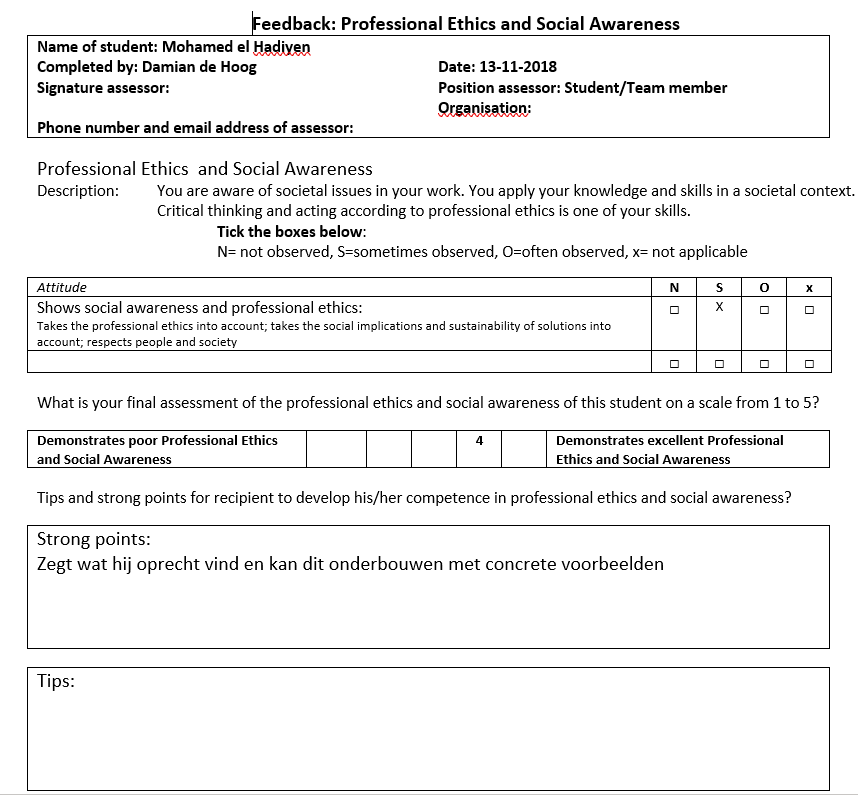
\includegraphics[width=\columnwidth]{ProfEthMohamed.PNG}\\
		\caption{Professional Ethics feedback Mohamed by Damian}
	\end{figure}
	\begin{figure}[p!]
		\centering
		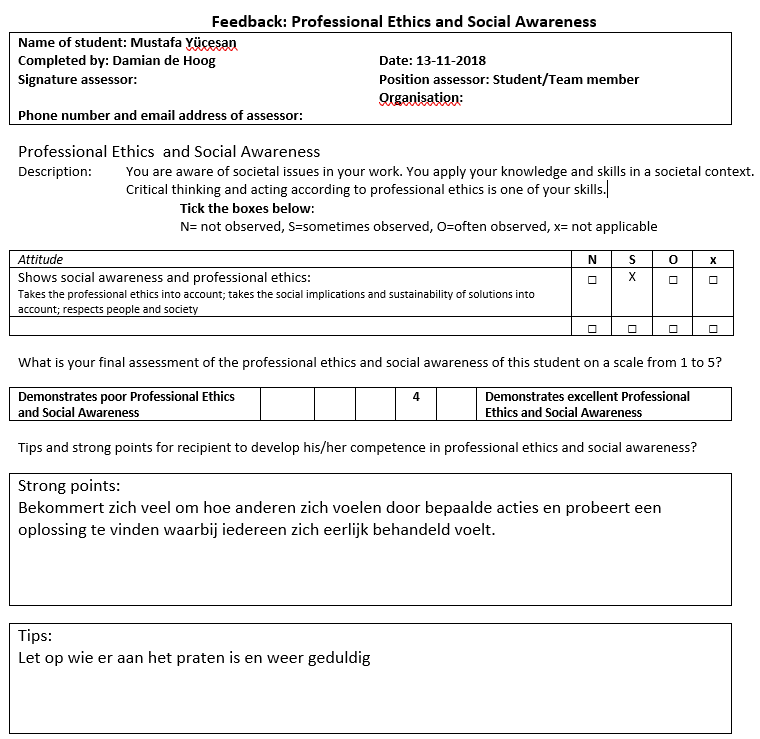
\includegraphics[width=\columnwidth]{ProfEthMustafa.PNG}\\
		\caption{Professional Ethics feedback Mustafa by Damian}
	\end{figure}
	\begin{figure}[p!]
		\centering
		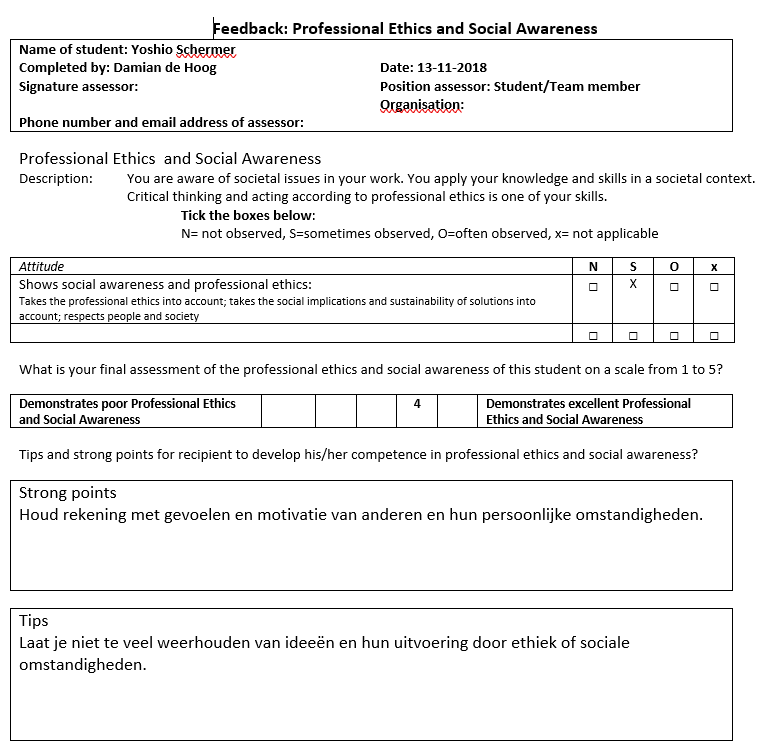
\includegraphics[width=\columnwidth]{ProfEthYoshio.PNG}\\
		\caption{Professional Ethics feedback Yoshio by Damian}
	\end{figure}
	\begin{figure}[p!]
		\centering
		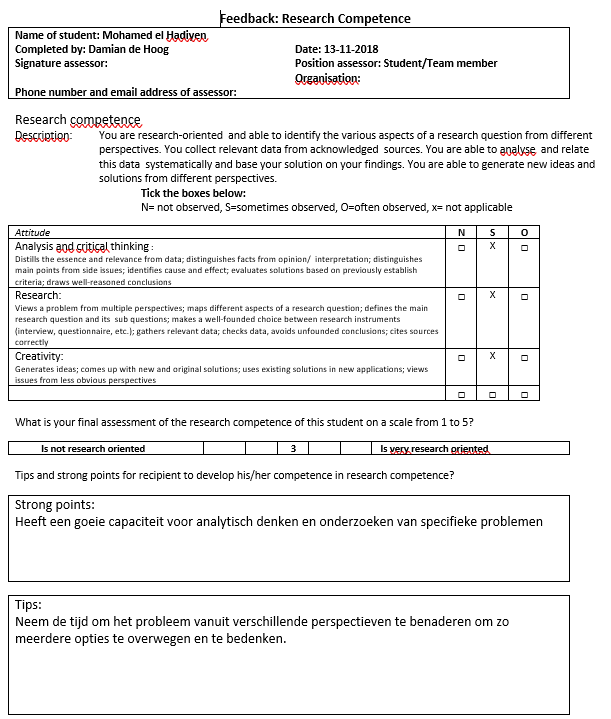
\includegraphics[width=\columnwidth]{ResSklMohamed.PNG}\\
		\caption{Research competence feedback Mohamed by Damian}
	\end{figure}
	\begin{figure}[p!]
		\centering
		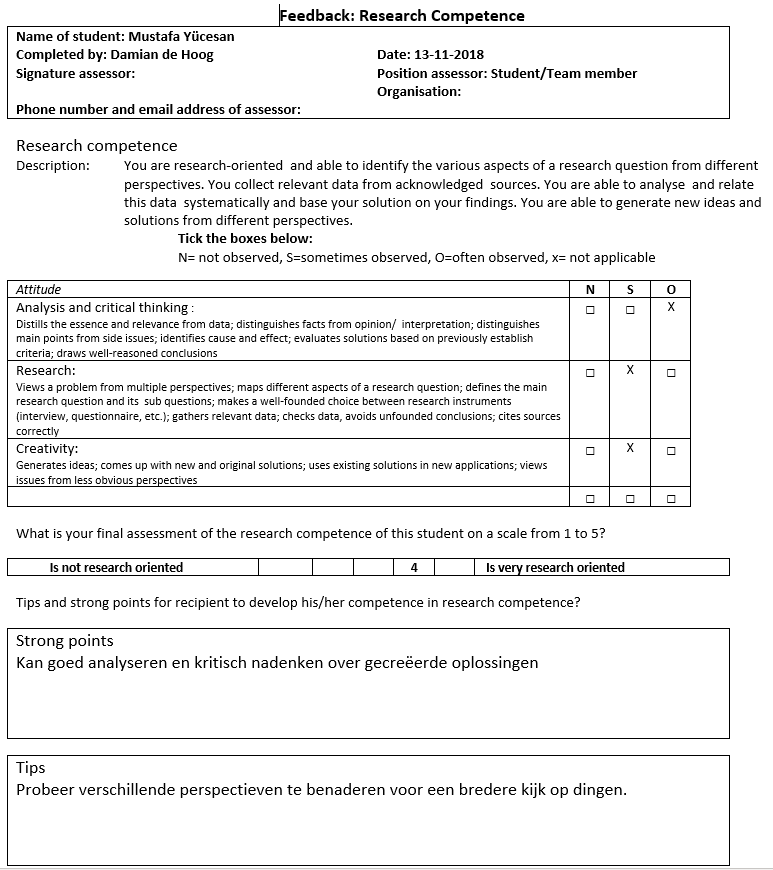
\includegraphics[width=\columnwidth]{ResSklMustafa.PNG}\\
		\caption{Research competence feedback Mustafa by Damian}
	\end{figure}
	\begin{figure}[p!]
		\centering
		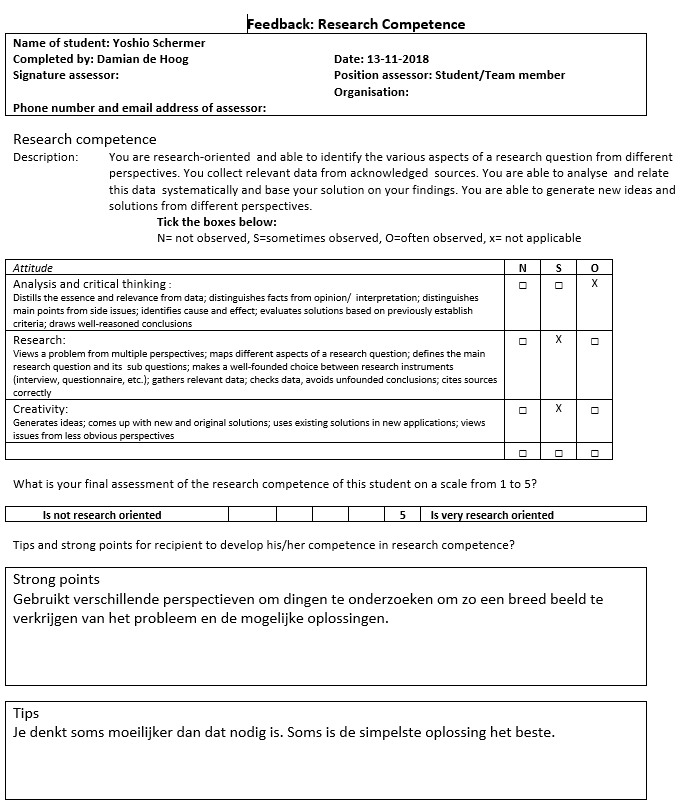
\includegraphics[width=\columnwidth]{ResSklYoshio.PNG}\\
		\caption{Research competence feedback Yoshio by Damian}
	\end{figure}
	\begin{figure}[p!]
		\centering
		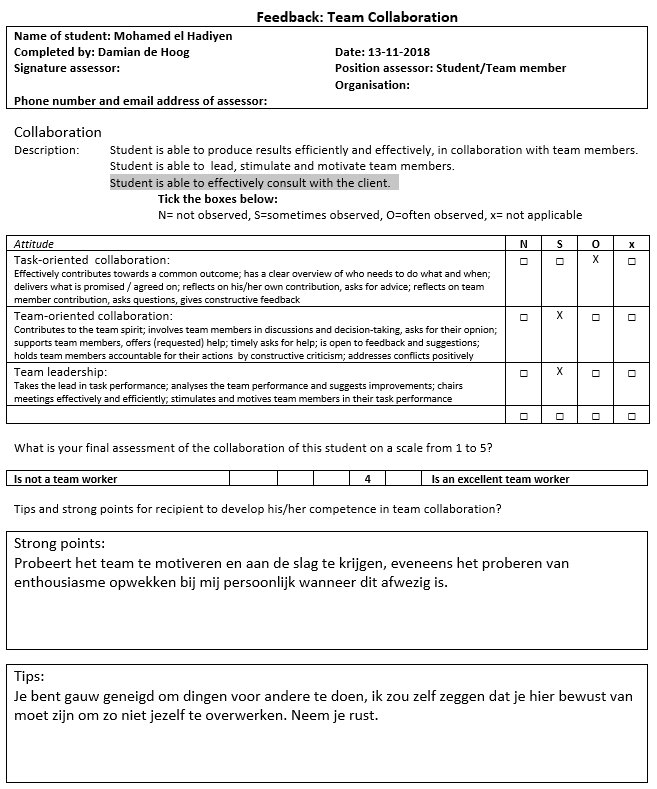
\includegraphics[width=\columnwidth]{CoopMohamed.PNG}\\
		\caption{Team Collaboration feedback Mohamed by Damian}
	\end{figure}
	\begin{figure}[p!]
		\centering
		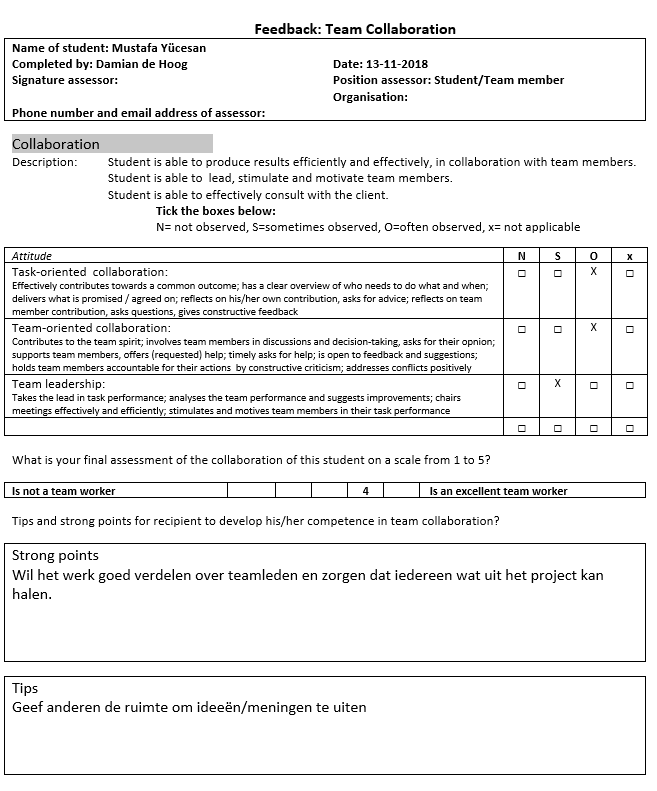
\includegraphics[width=\columnwidth]{CoopMustafa.PNG}\\
		\caption{Team Collaboration feedback Mustafa by Damian}
	\end{figure}
	\begin{figure}[p!]
		\centering
		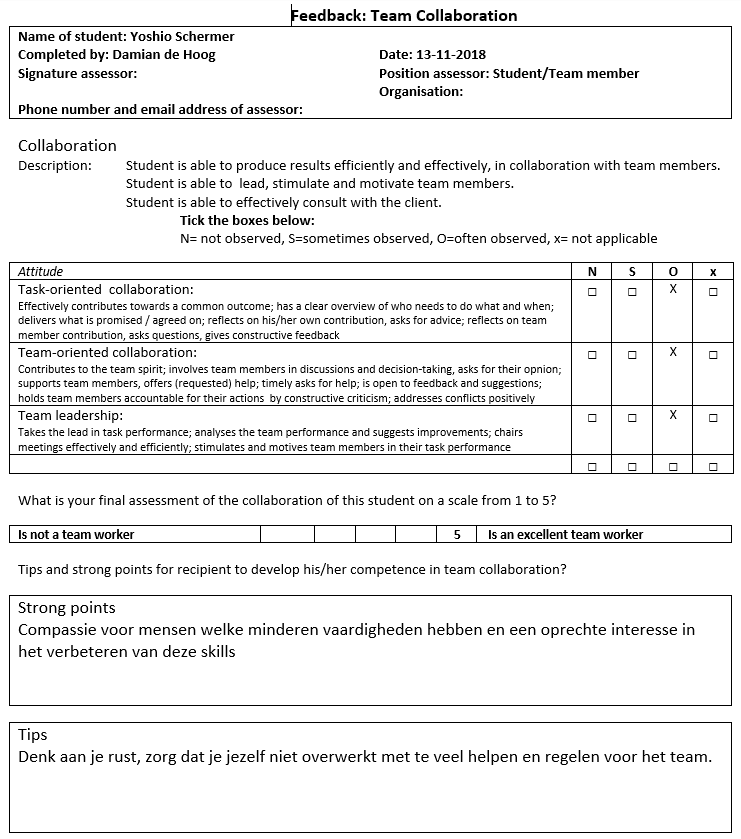
\includegraphics[width=\columnwidth]{CoopYoshio.PNG}\\
		\caption{Team Collaboration feedback Yoshio by Damian}
	\end{figure}
	\begin{figure}[p!]
		\centering
		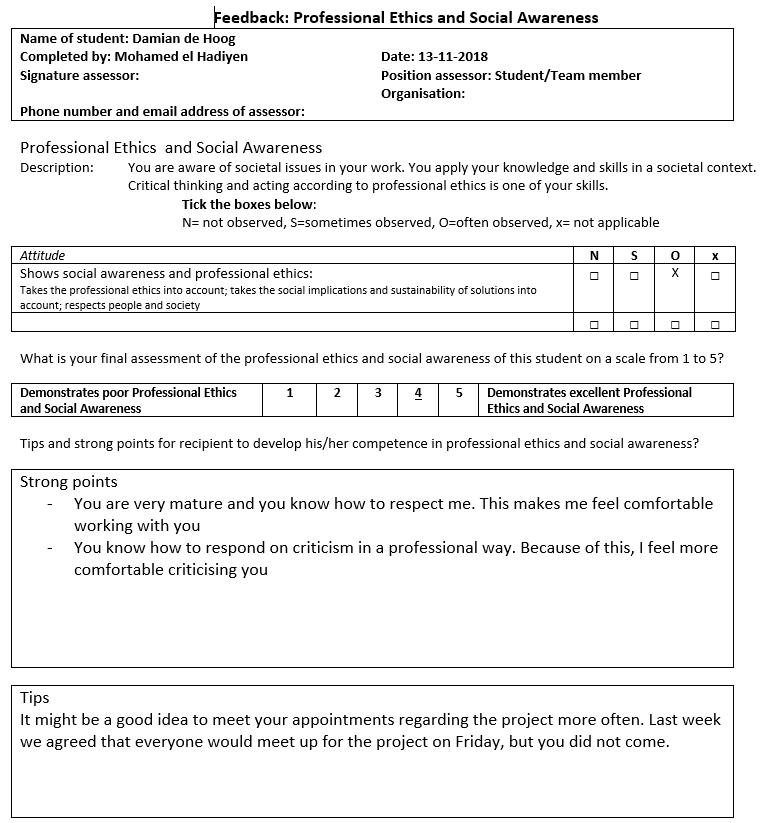
\includegraphics[width=\columnwidth]{ProfEthDamian1.PNG}\\
		\caption{Professional Ethics feedback Damian by Mohamed}
	\end{figure}
	\begin{figure}[p!]
		\centering
		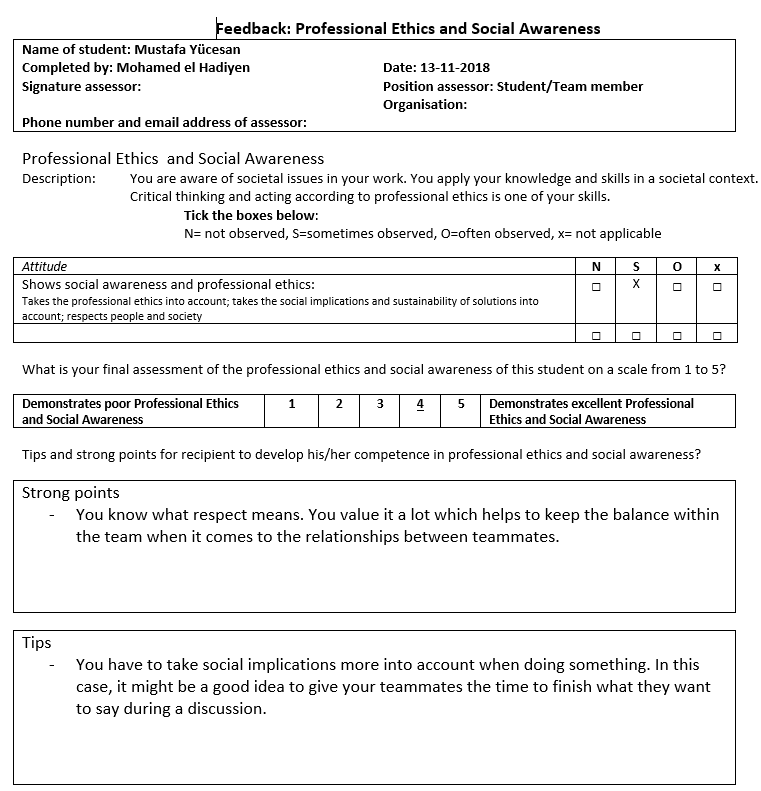
\includegraphics[width=\columnwidth]{ProfEthMustafa1.PNG}\\
		\caption{Professional Ethics feedback Mustafa by Mohamed}
	\end{figure}
	\begin{figure}[p!]
		\centering
		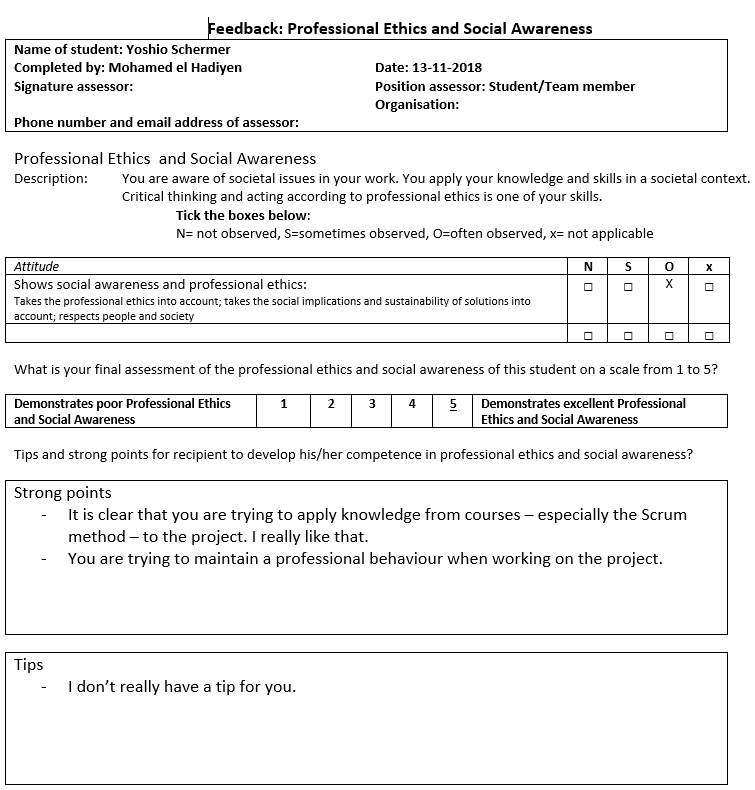
\includegraphics[width=\columnwidth]{ProfEthYoshio1.PNG}\\
		\caption{Professional Ethics feedback Yoshio by Mohamed}
	\end{figure}
	\begin{figure}[p!]
		\centering
		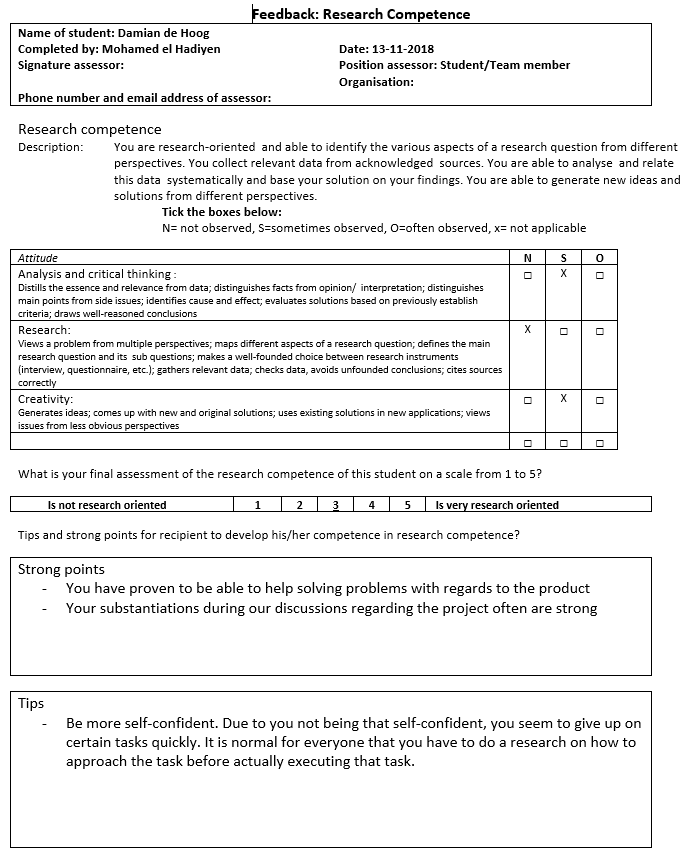
\includegraphics[width=\columnwidth]{ResSklDamian1.PNG}\\
		\caption{Research competence feedback Damian by Mohamed}
	\end{figure}
	\begin{figure}[p!]
		\centering
		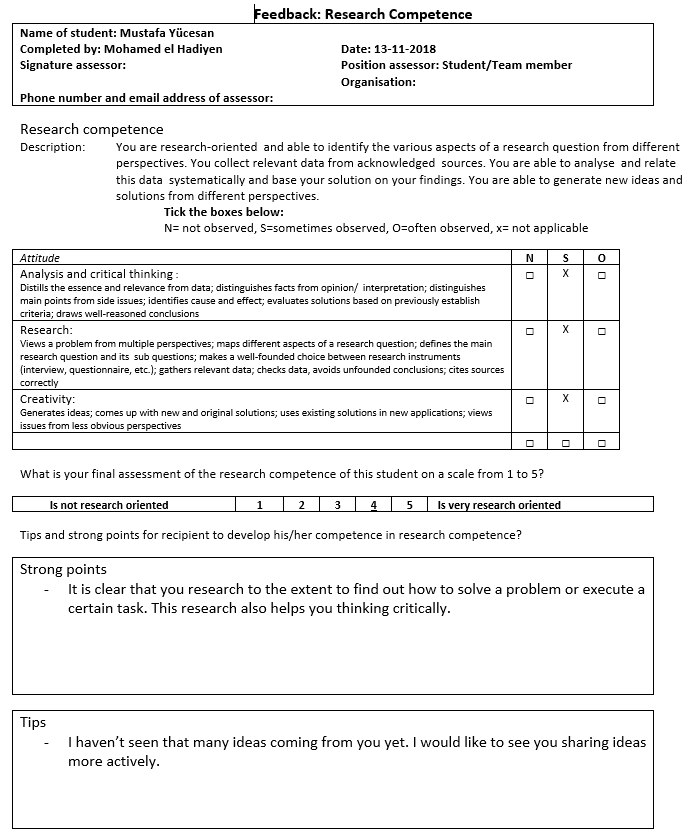
\includegraphics[width=\columnwidth]{ResSklMustafa1.PNG}\\
		\caption{Research competence feedback Mustafa by Mohamed}
	\end{figure}
	\begin{figure}[p!]
		\centering
		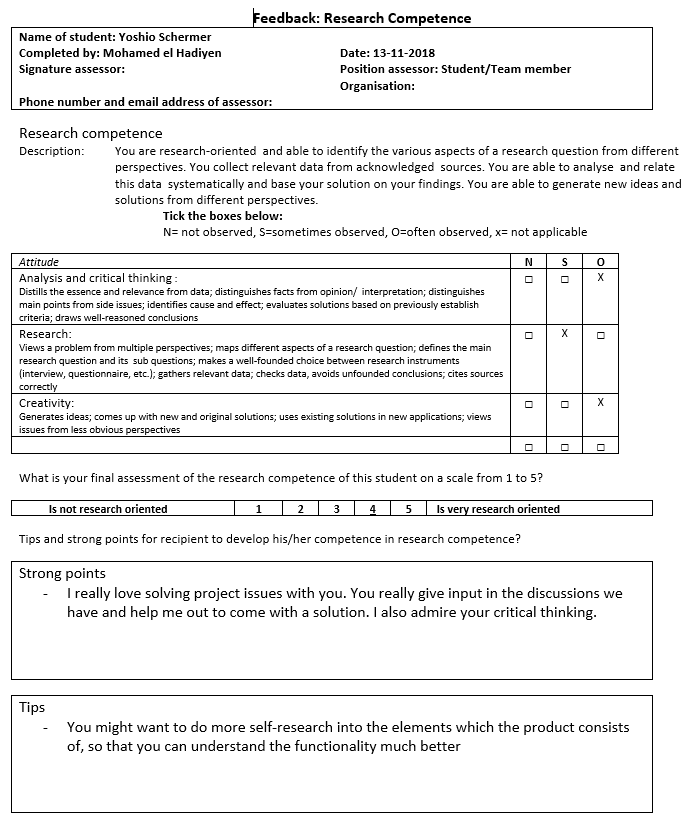
\includegraphics[width=\columnwidth]{ResSklYoshio1.PNG}\\
		\caption{Research competence feedback Yoshio by Mohamed}
	\end{figure}
	\begin{figure}[p!]
		\centering
		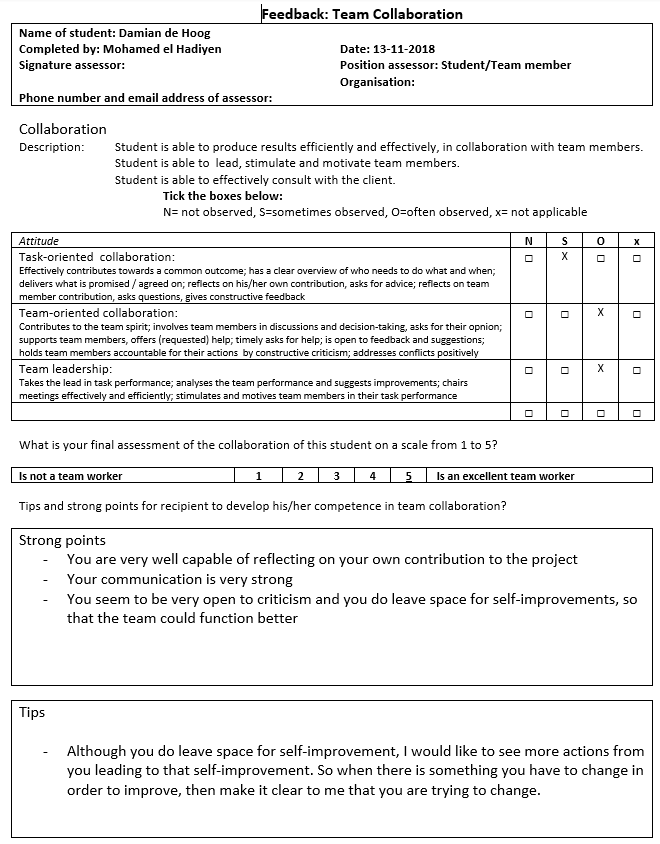
\includegraphics[width=\columnwidth]{CoopDamian1.PNG}\\
		\caption{Team Collaboration feedback Damian by Mohamed}
	\end{figure}
	\begin{figure}[p!]
		\centering
		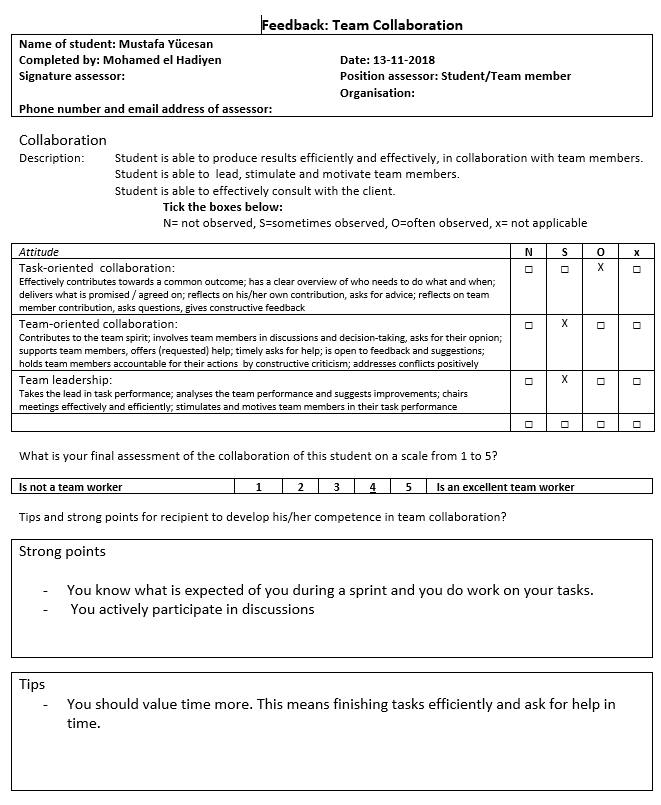
\includegraphics[width=\columnwidth]{CoopMustafa1.PNG}\\
		\caption{Team Collaboration feedback Mustafa by Mohamed}
	\end{figure}
	\begin{figure}[p!]
		\centering
		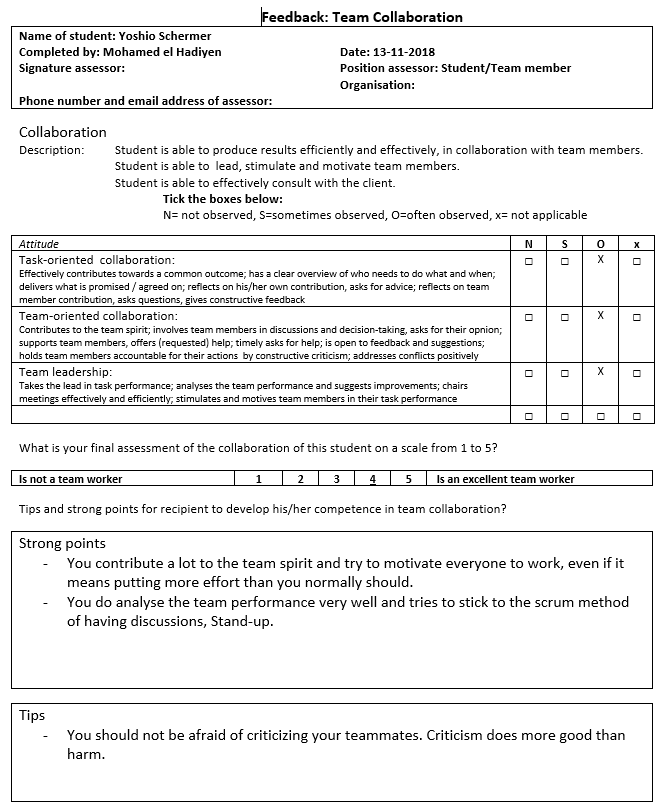
\includegraphics[width=\columnwidth]{CoopYoshio1.PNG}\\
		\caption{Team Collaboration feedback Yoshio by Mohamed}
	\end{figure}
	\begin{figure}[p!]
		\centering
		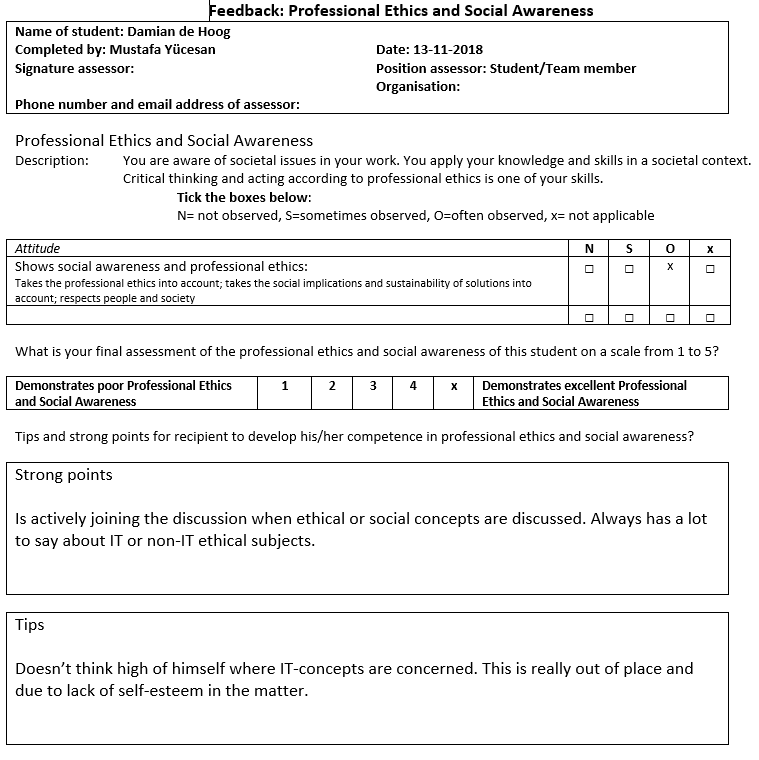
\includegraphics[width=\columnwidth]{ProfEthDamian2.PNG}\\
		\caption{Professional Ethics feedback Damian by Mustafa}
	\end{figure}
	\begin{figure}[p!]
		\centering
		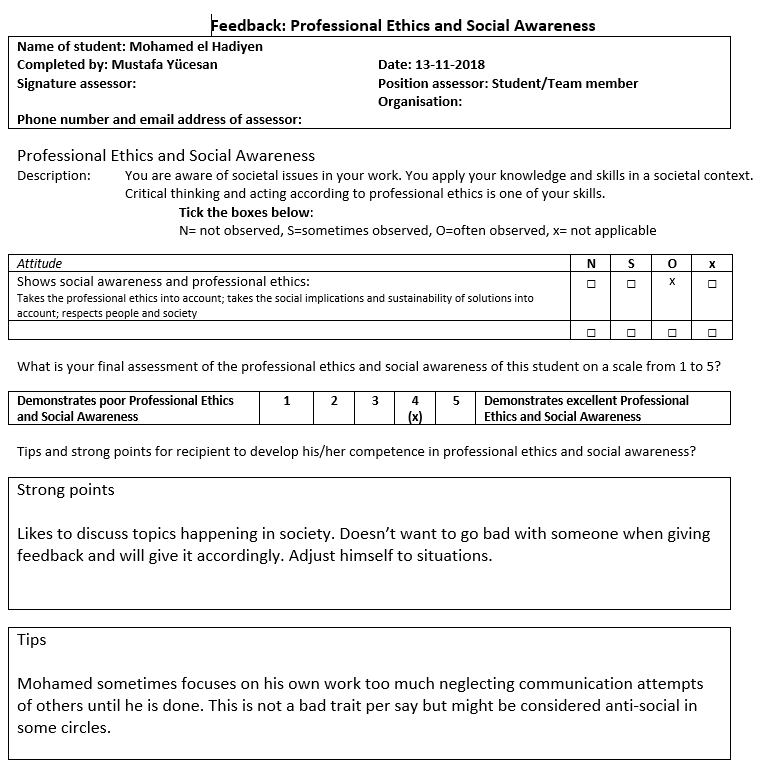
\includegraphics[width=\columnwidth]{ProfEthMohamed2.PNG}\\
		\caption{Professional Ethics feedback Mohamed by Mustafa}
	\end{figure}
	\begin{figure}[p!]
		\centering
		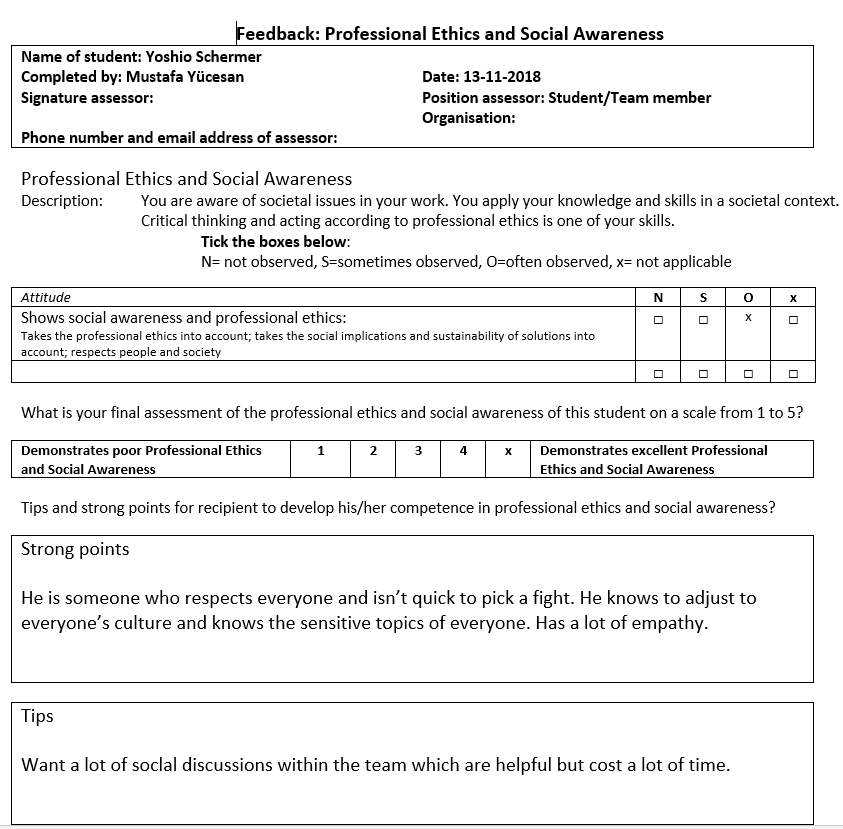
\includegraphics[width=\columnwidth]{ProfEthYoshio2.PNG}\\
		\caption{Professional Ethics feedback Yoshio by Mustafa}
	\end{figure}
	\begin{figure}[p!]
		\centering
		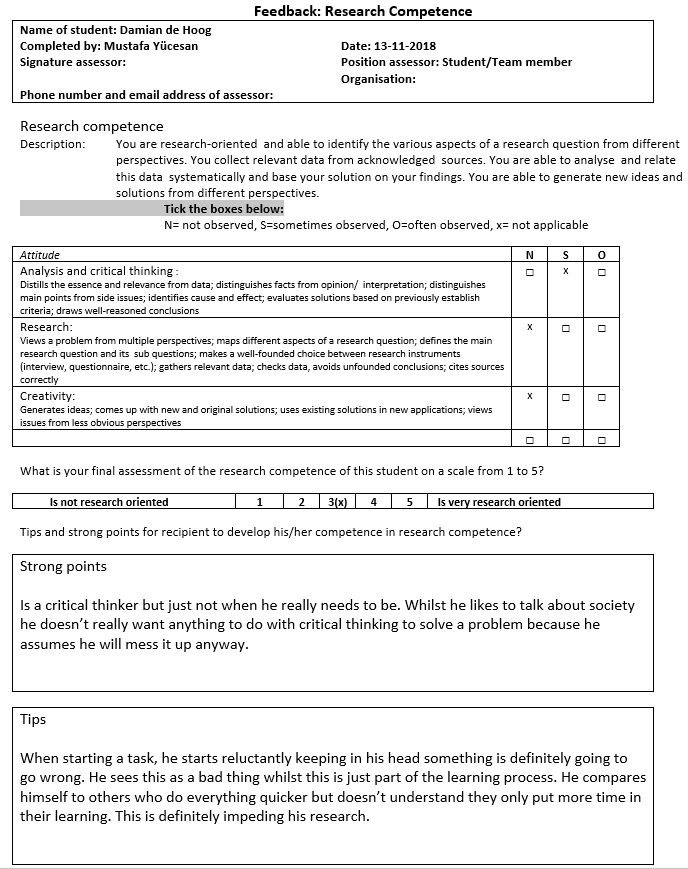
\includegraphics[width=\columnwidth]{ResSklDamian2.PNG}\\
		\caption{Research competence feedback Damian by Mustafa}
	\end{figure}
	\begin{figure}[p!]
		\centering
		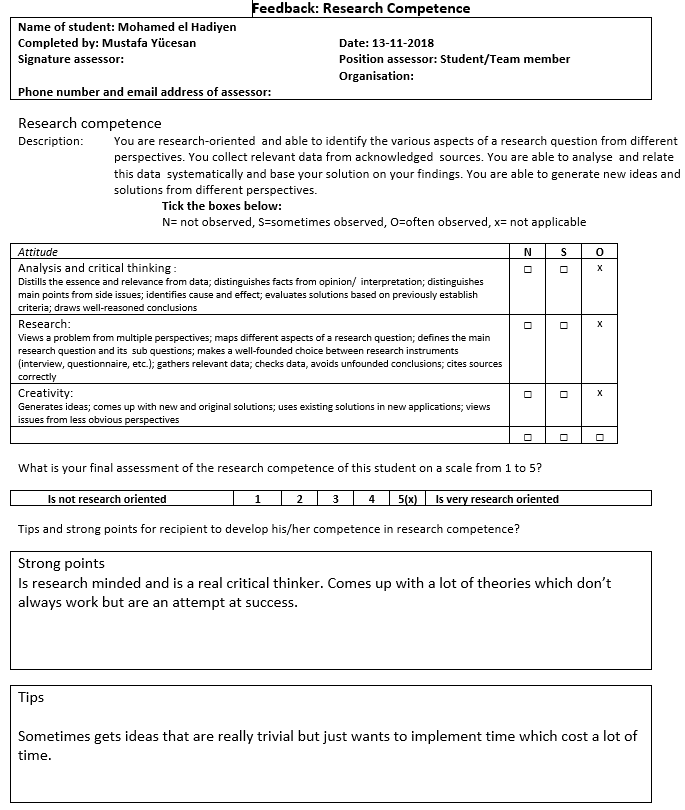
\includegraphics[width=\columnwidth]{ResSklMohamed2.PNG}\\
		\caption{Research competence feedback Mohamed by Mustafa}
	\end{figure}
	\begin{figure}[p!]
		\centering
		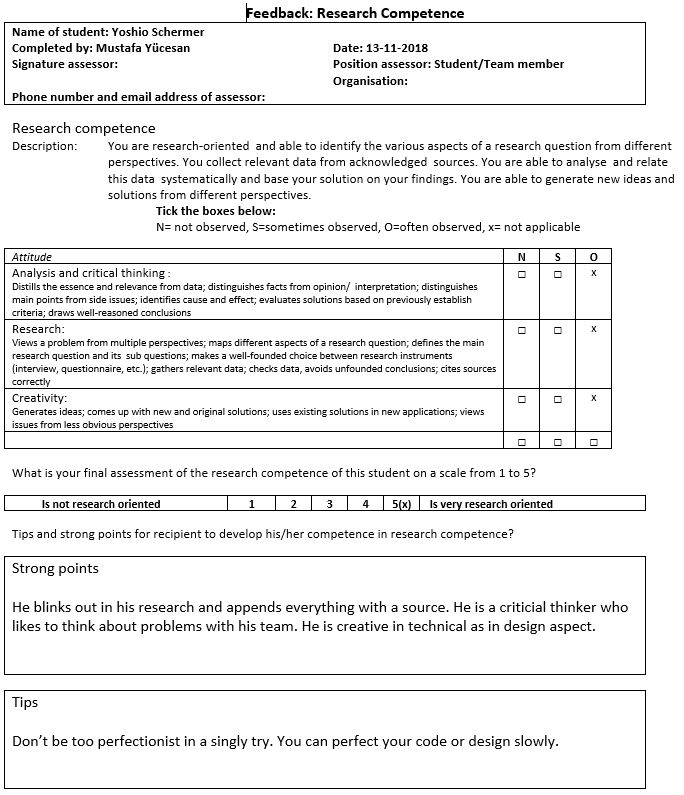
\includegraphics[width=\columnwidth]{ResSklYoshio2.PNG}\\
		\caption{Research competence feedback Yoshio by Mustafa}
	\end{figure}
	\begin{figure}[p!]
		\centering
		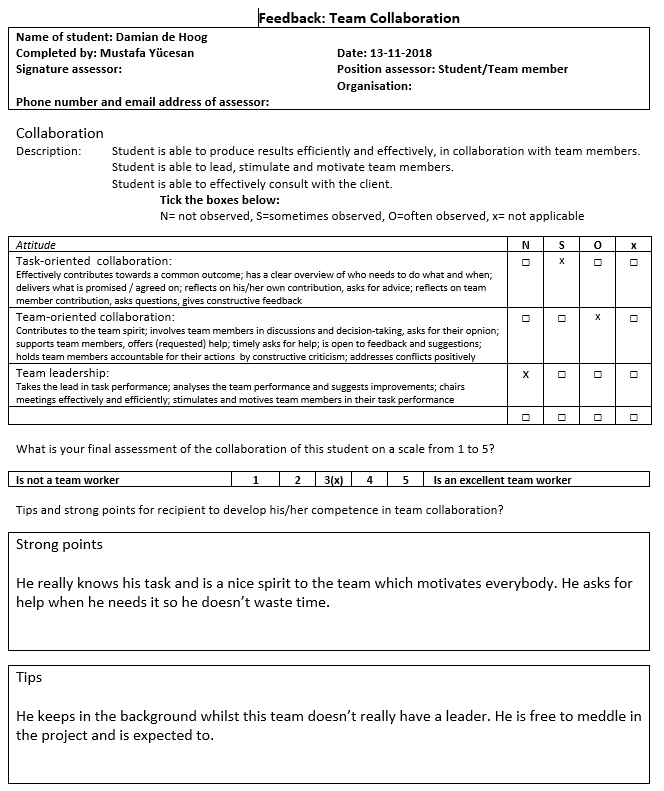
\includegraphics[width=\columnwidth]{CoopDamian2.PNG}\\
		\caption{Team Collaboration feedback Damian by Mustafa}
	\end{figure}
	\begin{figure}[p!]
		\centering
		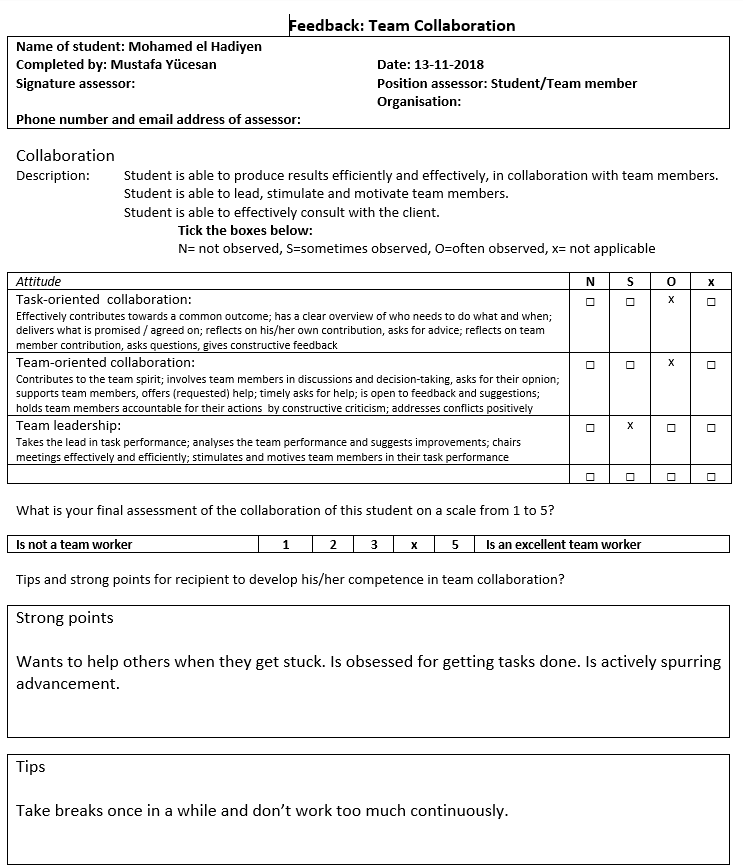
\includegraphics[width=\columnwidth]{CoopMohamed2.PNG}\\
		\caption{Team Collaboration feedback Mohamed by Mustafa}
	\end{figure}
	\begin{figure}[p!]
		\centering
		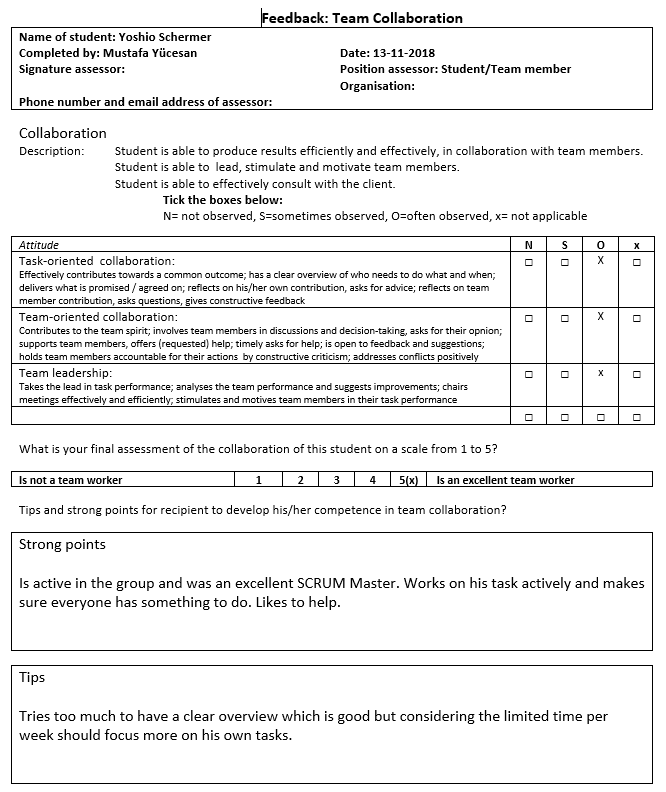
\includegraphics[width=\columnwidth]{CoopYoshio2.PNG}\\
		\caption{Team Collaboration feedback Yoshio by Mustafa}
	\end{figure}
	\begin{figure}[p!]
	\centering
	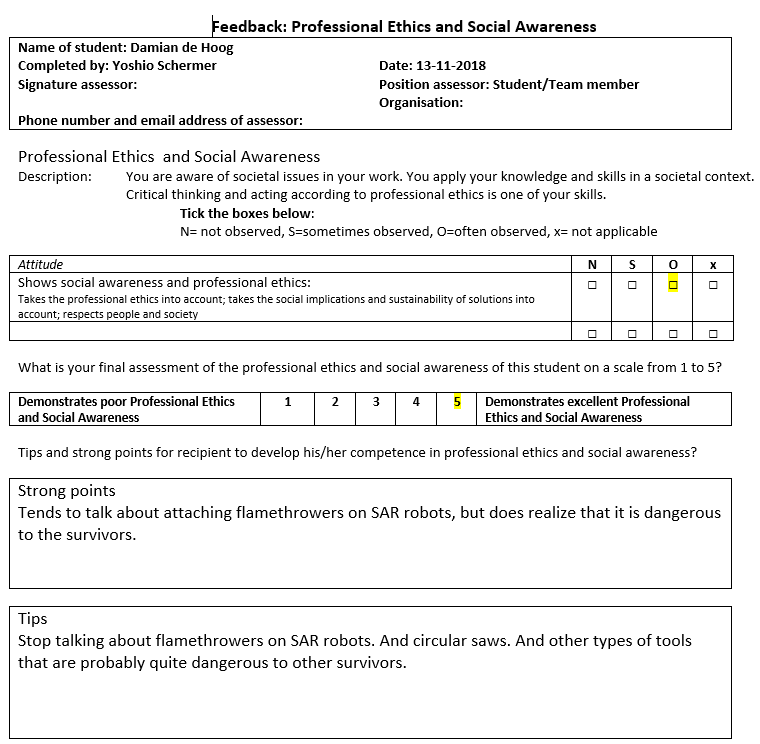
\includegraphics[width=\columnwidth]{ProfEthDamian3.PNG}\\
	\caption{Professional Ethics feedback Damian by Yoshio}
	\end{figure}
	\begin{figure}[p!]
		\centering
		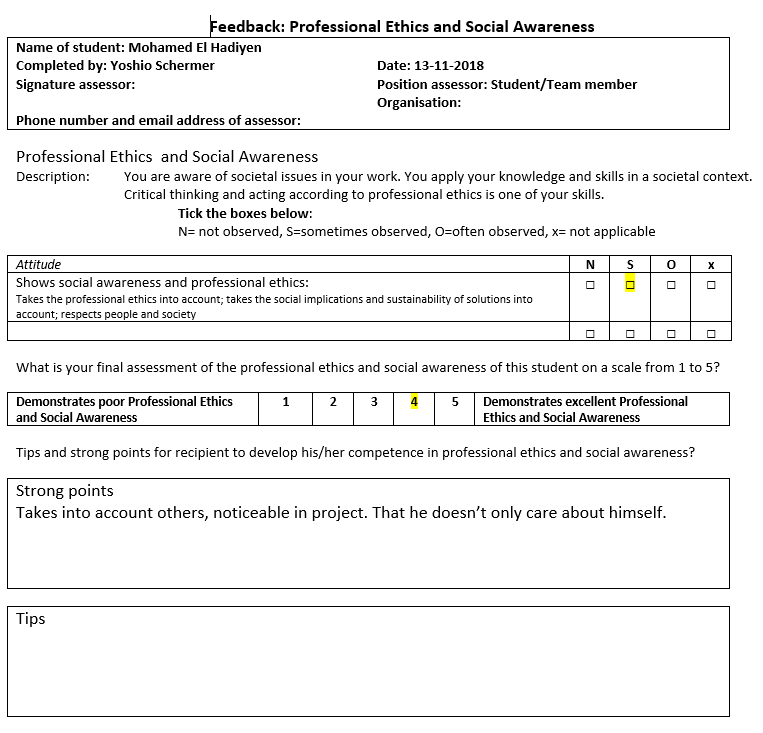
\includegraphics[width=\columnwidth]{ProfEthMohamed3.PNG}\\
		\caption{Professional Ethics feedback Mohamed by Yoshio}
	\end{figure}
	\begin{figure}[p!]
		\centering
		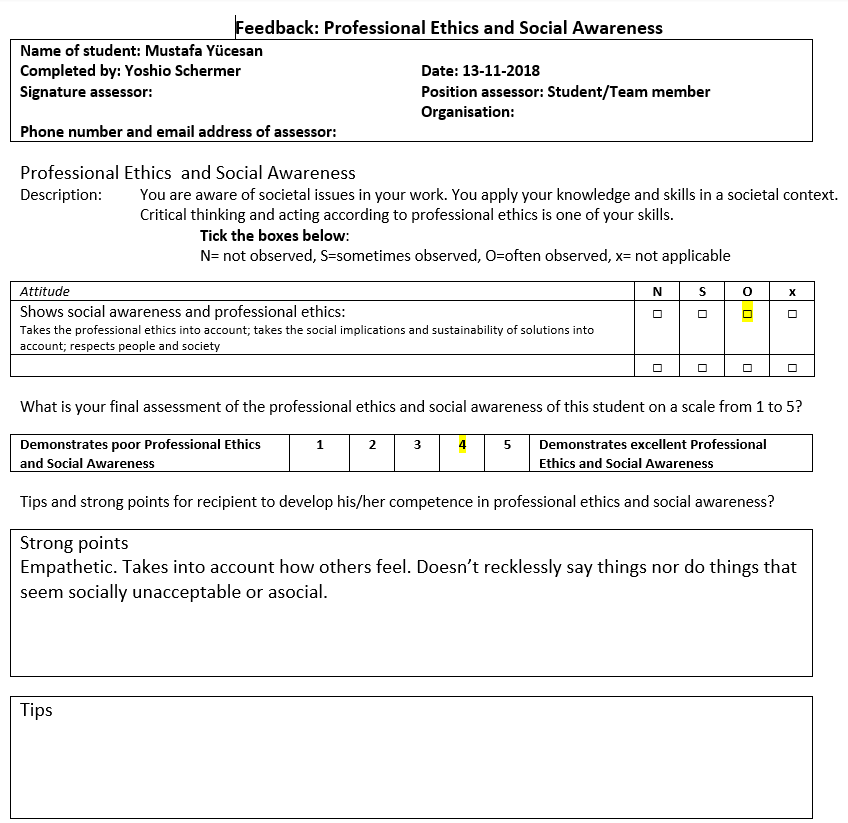
\includegraphics[width=\columnwidth]{ProfEthMustafa3.PNG}\\
		\caption{Professional Ethics feedback Mustafa by Yoshio}
	\end{figure}
	\begin{figure}[p!]
		\centering
		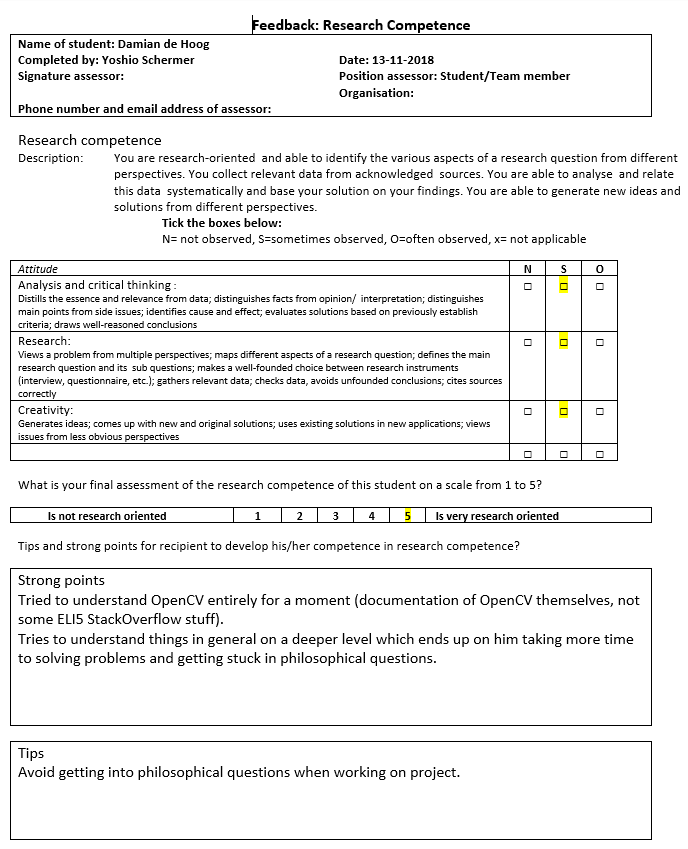
\includegraphics[width=\columnwidth]{ResSklDamian3.PNG}\\
		\caption{Research competence feedback Damian by Yoshio}
	\end{figure}
	\begin{figure}[p!]
		\centering
		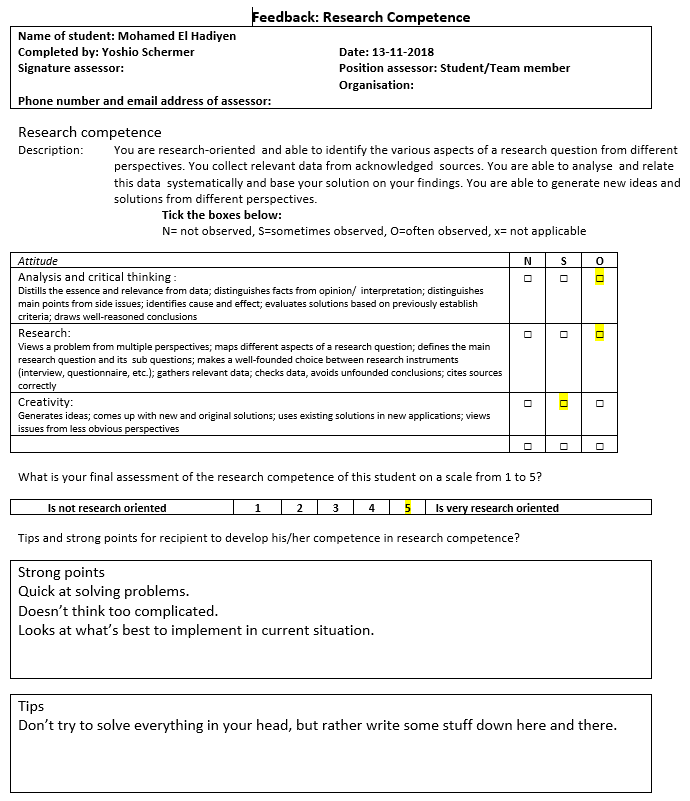
\includegraphics[width=\columnwidth]{ResSklMohamed3.PNG}\\
		\caption{Research competence feedback Mohamed by Yoshio}
	\end{figure}
	\begin{figure}[p!]
		\centering
		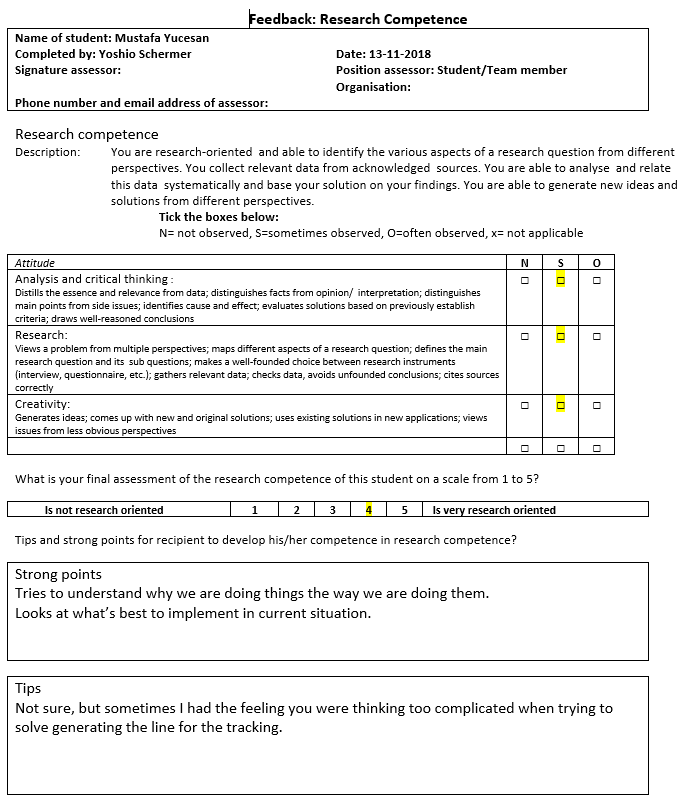
\includegraphics[width=\columnwidth]{ResSklMustafa3.PNG}\\
		\caption{Research competence feedback Mustafa by Yoshio}
	\end{figure}
	\begin{figure}[p!]
		\centering
		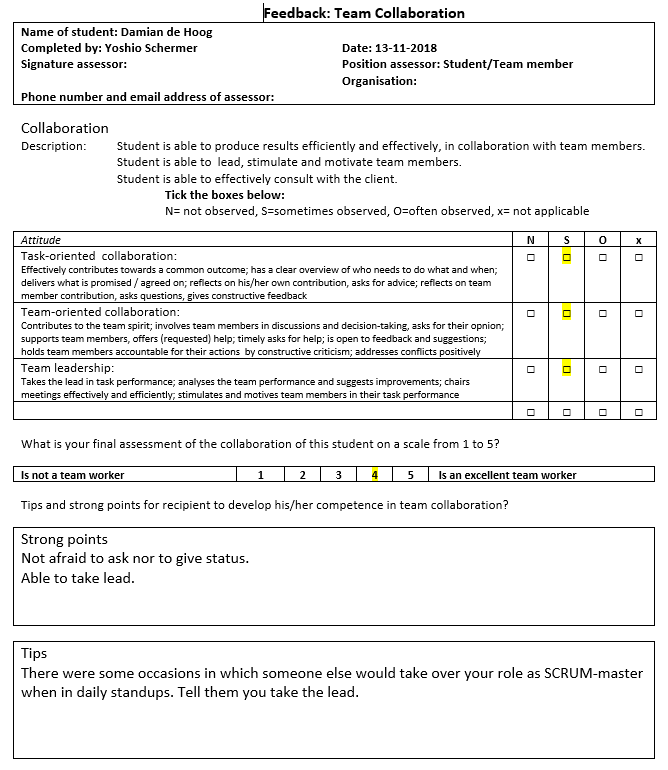
\includegraphics[width=\columnwidth]{CoopDamian3.PNG}\\
		\caption{Team Collaboration feedback Damian by Yoshio}
	\end{figure}
	\begin{figure}[p!]
		\centering
		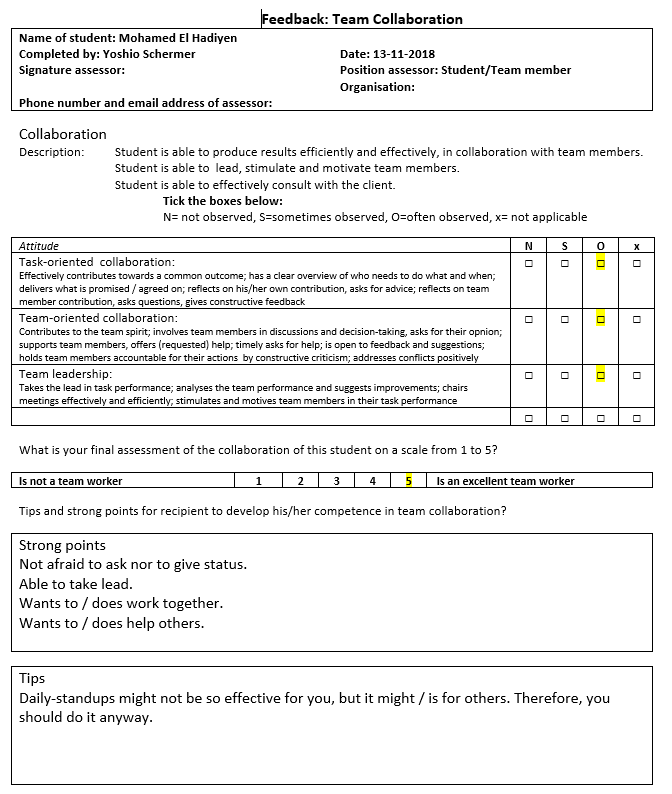
\includegraphics[width=\columnwidth]{CoopMohamed3.PNG}\\
		\caption{Team Collaboration feedback Mohamed by Yoshio}
	\end{figure}
	\begin{figure}[p!]
		\centering
		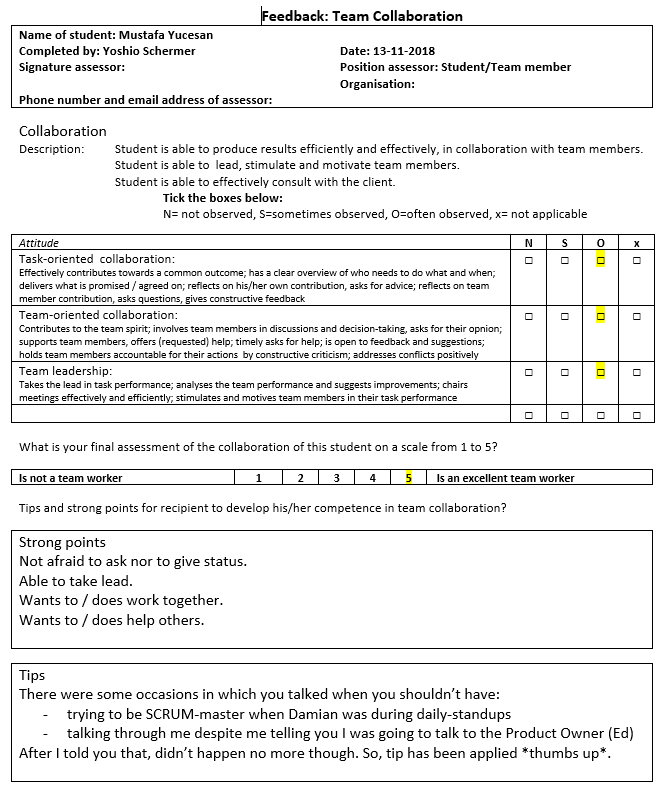
\includegraphics[width=\columnwidth]{CoopMustafa3.PNG}\\
		\caption{Team Collaboration feedback Mustafa by Yoshio}
	\end{figure}
	\newpage
	\section{Educational goals SMART}
	This chapter contains educational goals for each of our team members. These goals have been formulated according to the SMART methodology.
	These goals have been, where applicable, expanded upon with whether or not they have been successfully fulfilled or are in need of some more work.
	\subsection{Damian}
	\begin{itemize}
		\item Professioneel vakmanschap: At the end of the project I want to have scheduled a week and completed it with at least 75\% accuracy.
		\begin{itemize}
			\item Succes, the week of 19 november was completed with 92\% accuracy.
		\end{itemize}
		\item Onderzoekend vermogen: At the end of the project I want to at least have researched a way to implement one of the features of our product.
		\begin{itemize}
			\item Succes, LCD screen implementation. 
		\end{itemize}
		\item Leervermogen: During this project I want to study myself and try and figure out why I keep postponing schoolwork.
		\begin{itemize}
			\item Succes, Observed several factors contributing to the behaviour. 
		\end{itemize}
		\item Communicatief vermogen: During this project I want to improve the communication between me and my team members in comparison to PAD. This means, healthy discussions and no avoidance of interaction.
		\begin{itemize}
			\item Successful so far.
		\end{itemize}
		\item Beroepsethiek en maatschappelijke oriëntatie: During this project I want to refrain from implementing unethical features.
		\begin{itemize}
			\item Succes, Flamethrower was not implemented.
		\end{itemize}
		\item Samenwerken: During this project I want to try not miss any scheduled project workdays at school.
		\begin{itemize}
			\item Failed, missed one day so far. Reflection upon this missed day has led to prevention of more missed days.
		\end{itemize}
	\end{itemize}
	\subsection{Mohamed}
	\begin{itemize}
		\item Professioneel vakmanschap: During this project, I am able to put the theory I have learnt during the lessons from Technical Computing into practice on the rover.
		\begin{itemize}
			\item Success, Implementation of the Singleton pattern.
		\end{itemize}
		\item Onderzoekend vermogen: During this project, I will research software patterns so that I can write efficient code.
		\begin{itemize}
			\item Success, researched the adaptability and implementation of the Singleton pattern within our own project. 
		\end{itemize}
		\item Leervermogen: At the end of Robot On Wheels Project, I - with the help of my motivation - have learned how to reflect on my development in a project.
		\begin{itemize}
			\item Success, self reflection during the retrospectives and stand-ups.
		\end{itemize}
		\item Communicatief vermogen: During the last presentation for Robot On Wheels Project, I will be able to speak English more fluent.
		\begin{itemize}
			\item Not yet successful, maybe more speaking during the presentations.
		\end{itemize}
		\item Beroepsethiek en maatschappelijke oriëntatie: For this project, I will create a rover which meets the user guideline Usability.
		\begin{itemize}
			\item Not yet successful, will be covered during the final sprint when focus is put on the perception of our product in terms of usability.
		\end{itemize}
		\item Samenwerken: After the first sprint of Robot On wheels Project, I will be able to trust my colleagues hand out tasks with confidence.
		\begin{itemize}
			\item Successful, I have been able to give my teammates tasks without staying involved for example: Damian and the ultrasonic sensor.
		\end{itemize}
	\end{itemize}
	\subsection{Mustafa}
	\begin{itemize}
		\item Professioneel vakmanschap: At the end of the project I want to be a specialist in IT-projects and this will be measured by the perceived (by team members) performance and specialty.  
		\begin{itemize}
			\item My goal has partially been reached but it can be much better.
		\end{itemize}
		\item Onderzoekend vermogen: I want to have faster and more efficient research methods for information that I need by the end of this year. This will be measured by analytical documents made during the project.
		\begin{itemize}
			\item Didn't work because the analytical documents have not been made yet.
		\end{itemize}
		\item Leervermogen: I want to improve my learning capacity in such a way that I can solve problems and learn from it by the end of the project. This will be measured by a reflection at the end of the project.
		\begin{itemize}
			\item Didn't work because we didn't have any reflection yet.
		\end{itemize}
		\item Communicatief vermogen: 
		I want to be more adept at presentations in general but specifically in English by the end of the year. This will be measured at the sprint reviews.
		\begin{itemize}
			\item 	Worked, I received positive feedback from the teacher with B2 English. I myself notice improvement.
		\end{itemize} 
		\item Beroepsethiek en maatschappelijke oriëntatie: By the end of the year I would like to have a better comprehension of the position of Technical Computing within our society. This will be measured by my attendance at ethical lectures.
		\begin{itemize}
			\item Did work, I have a much better comprehension now.
		\end{itemize}
		\item Samenwerken: I would like to be better at teamwork with my colleagues to achieve a beautiful result at the end of the project. 
		\begin{itemize}
			\item Worked partly. The team is divided between two parties. One things we have managed a lot but the others lack the quality to realise that. I believe it is the toxic effect of perfectionism. We do get a proper result but one party doesn't know how to pat themselves on the back.  
		\end{itemize}
	\end{itemize}
	\subsection{Yoshio}
	\begin{itemize}
		\item Professioneel vakmanschap
		In this project I will regularly communicate with the product owner concerning the project.
		\begin{itemize}
			\item Success, correspondence with the prodcut owner has been documented on google drive and implemented in a later chapter inside this document. 
		\end{itemize}
		\item Onderzoekend vermogen
		In this project I want to make a document describing the days/weeks that team members are (un)available and when the probability that they’re busy or sick is high/low, so we can adjust our Sprints to this.
		\begin{itemize}
			\item Success, uploaded on google drive ( Link at the start of this document, Tools).
		\end{itemize}
		\item Leervermogen
		At the end of this project I will have obtained, from my team members through interviewing them, at least 3 strengths and 3 weaknesses that I didn’t know before of.
		\begin{itemize}
			\item Working on it, missing a few points from Damian and Mohamed.
		\end{itemize}
		\item Communicatief vermogen
		At the end of this project I will interview the product owner about my performance as a product owner delegate so I can see what I could improve/did well.
		\begin{itemize}
			\item Project has not ended as of writing this.
		\end{itemize}
		\item Beroepsethiek en maatschappelijke oriëntatie
		At the end of this project I will document at least one possible implementation and describe that it’s unethical to implement.
		\begin{itemize}
			\item Success, uploaded to our google drive.
		\end{itemize}
		\item Samenwerken
		In this project I will ask members of the team how they’re doing personally so I can adjust my attitude towards their situation.
		\begin{itemize}
			\item Success, I stay involved with the well being of my teammates, for example: Mustafa and his dentist appointment for a tooth problem.
		\end{itemize}
	\end{itemize}
	\newpage
	\section{Feedback based educational goals}
	This chapter also contains educational goals, however, these have been formulated based on the feedback supplied by each team member through the feedback forms. These goals have been formed recently and thus have not provided with the results of efforts made towards them.
	\subsection{Damian}
	\begin{itemize}
		\item Based on the feedback supplied by my team members I conclude that I have to be more confident in my IT skills and be less harsh on myself when I hit an obstacle or fail. Failing is part of the learning process and everything I fail now, I destroy my self image with words of discouragement.
		\item Based on the feedback supplied by my team members I conclude that I have to be more actively engaged with the project. Due to motivational problems and lack of interest I find it hard to be fully engaged with the project. This is not a new problem to me personally. I have to figure out how to stay conscious of this and actively work towards my goal.
	\end{itemize}
	\subsection{Mohamed}
	\begin{itemize}
		\item Based on the feedback supplied by my team members I conclude that I should take more time considering how to approach a certain issue/task in the project. Apparently I rush in working on my tasks. I can understand this, so I am going to invest more time in thinking of the approach, and I will be using Trello to note down my issues and how I have solved them.
		\item Based on the feedback supplied by my team members I conclude that I should not work overtime. I do invest extra time into the project at home, because I really want to finish my tasks as fast as possible, so that I can go to the next task. However, this seems to have bad consequences for me, so I will be taking more breaks and plan my time working for the project better.		
	\end{itemize}
	\subsection{Mustafa}
	\begin{itemize}
		\item Based on the feedback supplied by my team members I will try not to over-complicate things so I become a quicker problem solver. My teammates will tell me if I managed.
		\item Based on the feedback supplied by my team members I will try to look at problems with different perspectives so I have a wider view of things. My teammates will tell me if I managed.
	\end{itemize}
	\subsection{Yoshio}
	\begin{itemize}
		\item Based on the feedback supplied by my team members I will decrease the time spent on discussing things. At the end of the project, I will ask the team to evaluate whether I have done so. Also more importantly, whether this made the team more productive.
		\item Based on the feedback supplied I will let my team members evaluate me at the end of the project on whether I have taken on more an attitude of productivity versus perfectionism.
	\end{itemize}
	\newpage
	\section{Daily stand-ups}
	The following chapters contain notes from team activities, starting with the notes from our Scrum daily stand-ups. These stand-ups are like small progress meetings to see whether everyone has a task or knows what he should be doing, if anyone has encountered any problems and if anyone needs help with their tasks.\\
	The notes from these meetings have been ordered chronologically and are the same as found on our wordpress blog ( Link at the start of the document, tools).
	\paragraph{Daily stand-up 17 \& 18 September}
	SCRUM-master: Damian\\
	\\\textbf{How are things going so far?}
	\begin{itemize}
		\item Problems with the hardware have mostly been solved. The magnetometer doesn't work, according to Ruud this will be discussed later on in the project.
		\item During classes we can see how other groups in class are performing, they seem to have made more progress than we have. This could be because the rover and it's movement aren't hard to program or other teams have spend a significant amount of time more on their product than we have.
	\end{itemize}
	\textbf{Wat hebben we gedaan?}
	\begin{itemize}
		\item Verbinden met de RPI en internet regelen voor de RPI.
		\item Mini-rover laten rijden m.b.v. Python vertaald uit C.
		\item Epics, user stories, use cases opgesteld.
		\item Samenwerkingsovereenkomst opgesteld.
		\item Blog (WordPress) gemaakt voor het bijhouden van standups, etc.
	\end{itemize}
	\textbf{Wat gaan we doen?}
	\begin{itemize}
		\item Coaching-afspraak regelen met Marten (Mustafa).
		\item C code  ombouwen naar Python (Mohamed \& Mustafa).
		\item Camera stream naar de browser (Damian).
		\item Camera stream naar de app (Damian \& Yoshio).
		\item Besturing via een extern apparaat (Mohamed).
		\item Design voor rover (Yoshio).
		\item Wifi-hotspot op de RPI (Yoshio).
	\end{itemize}
	
	
	\section{Coaching}
	\section{Retrospectives}
	\section{Impediments}
	\section{Communication with the product owner}
\end{document}	